\documentclass[]{article}
\usepackage{lmodern}
\usepackage{amssymb,amsmath}
\usepackage{ifxetex,ifluatex}
\usepackage{fixltx2e} % provides \textsubscript
\ifnum 0\ifxetex 1\fi\ifluatex 1\fi=0 % if pdftex
  \usepackage[T1]{fontenc}
  \usepackage[utf8]{inputenc}
\else % if luatex or xelatex
  \ifxetex
    \usepackage{mathspec}
  \else
    \usepackage{fontspec}
  \fi
  \defaultfontfeatures{Ligatures=TeX,Scale=MatchLowercase}
\fi
% use upquote if available, for straight quotes in verbatim environments
\IfFileExists{upquote.sty}{\usepackage{upquote}}{}
% use microtype if available
\IfFileExists{microtype.sty}{%
\usepackage{microtype}
\UseMicrotypeSet[protrusion]{basicmath} % disable protrusion for tt fonts
}{}
\usepackage[margin=1in]{geometry}
\usepackage{hyperref}
\hypersetup{unicode=true,
            pdftitle={Warfarin Pharmacy Dosing Service Analysis},
            pdfauthor={Brian Gulbis, PharmD, BCPS},
            pdfborder={0 0 0},
            breaklinks=true}
\urlstyle{same}  % don't use monospace font for urls
\usepackage{longtable,booktabs}
\usepackage{graphicx,grffile}
\makeatletter
\def\maxwidth{\ifdim\Gin@nat@width>\linewidth\linewidth\else\Gin@nat@width\fi}
\def\maxheight{\ifdim\Gin@nat@height>\textheight\textheight\else\Gin@nat@height\fi}
\makeatother
% Scale images if necessary, so that they will not overflow the page
% margins by default, and it is still possible to overwrite the defaults
% using explicit options in \includegraphics[width, height, ...]{}
\setkeys{Gin}{width=\maxwidth,height=\maxheight,keepaspectratio}
\IfFileExists{parskip.sty}{%
\usepackage{parskip}
}{% else
\setlength{\parindent}{0pt}
\setlength{\parskip}{6pt plus 2pt minus 1pt}
}
\setlength{\emergencystretch}{3em}  % prevent overfull lines
\providecommand{\tightlist}{%
  \setlength{\itemsep}{0pt}\setlength{\parskip}{0pt}}
\setcounter{secnumdepth}{0}
% Redefines (sub)paragraphs to behave more like sections
\ifx\paragraph\undefined\else
\let\oldparagraph\paragraph
\renewcommand{\paragraph}[1]{\oldparagraph{#1}\mbox{}}
\fi
\ifx\subparagraph\undefined\else
\let\oldsubparagraph\subparagraph
\renewcommand{\subparagraph}[1]{\oldsubparagraph{#1}\mbox{}}
\fi
\usepackage{float}

%%% Use protect on footnotes to avoid problems with footnotes in titles
\let\rmarkdownfootnote\footnote%
\def\footnote{\protect\rmarkdownfootnote}

%%% Change title format to be more compact
\usepackage{titling}

% Create subtitle command for use in maketitle
\newcommand{\subtitle}[1]{
  \posttitle{
    \begin{center}\large#1\end{center}
    }
}

\setlength{\droptitle}{-2em}
  \title{Warfarin Pharmacy Dosing Service Analysis}
  \pretitle{\vspace{\droptitle}\centering\huge}
  \posttitle{\par}
  \author{Brian Gulbis, PharmD, BCPS}
  \preauthor{\centering\large\emph}
  \postauthor{\par}
  \predate{\centering\large\emph}
  \postdate{\par}
  \date{June 2016}

\begin{document}
\maketitle

\subsection{Service Utilization}\label{service-utilization}

\subsubsection{Annual Warfarin
Utilization}\label{annual-warfarin-utilization}

\begin{figure}[H]
\centering
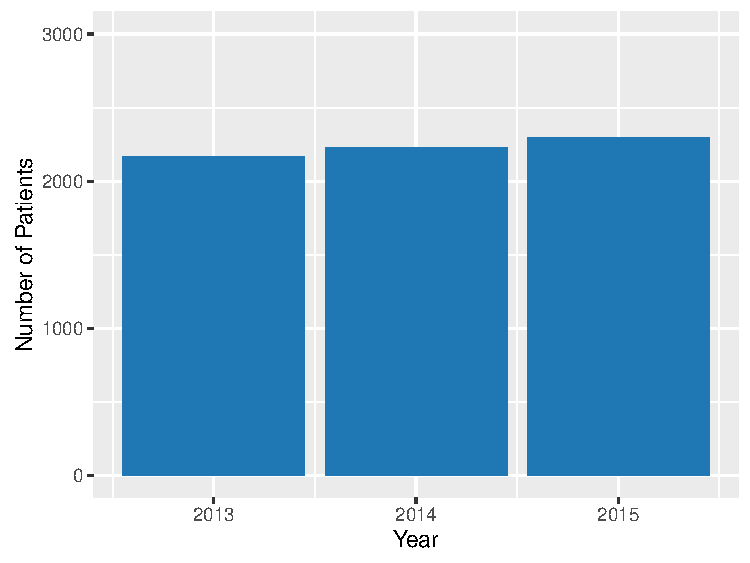
\includegraphics{warfarin_analysis_ASHP_files/figure-latex/graph_utilization-1.pdf}
\caption{Number of Patients Receiving Warfarin at MH-TMC, 2013-2015}
\end{figure}

\subsubsection{Utilization of Pharmacy Dosing
Service}\label{utilization-of-pharmacy-dosing-service}

\begin{figure}[H]
\centering
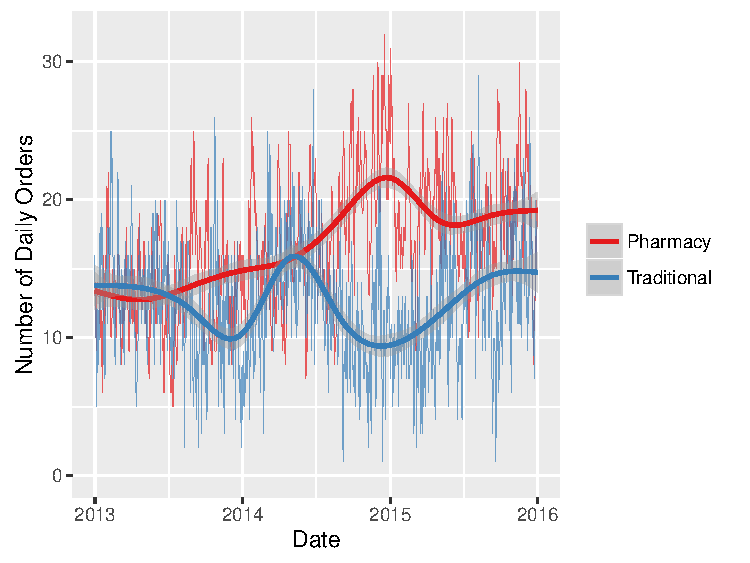
\includegraphics{warfarin_analysis_ASHP_files/figure-latex/dose_service_use-1.pdf}
\caption{Daily Warfarin Orders Managed by Pharmacy and Traditional}
\end{figure}

\begin{figure}[H]
\centering
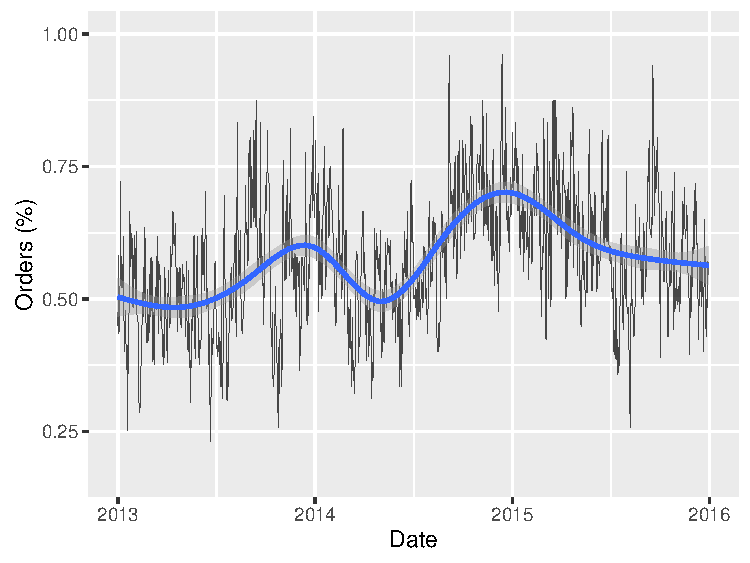
\includegraphics{warfarin_analysis_ASHP_files/figure-latex/dose_service_use2-1.pdf}
\caption{Percent of Daily Warfarin Orders Managed by Pharmacy Dosing
Service}
\end{figure}

\begin{figure}[H]
\centering
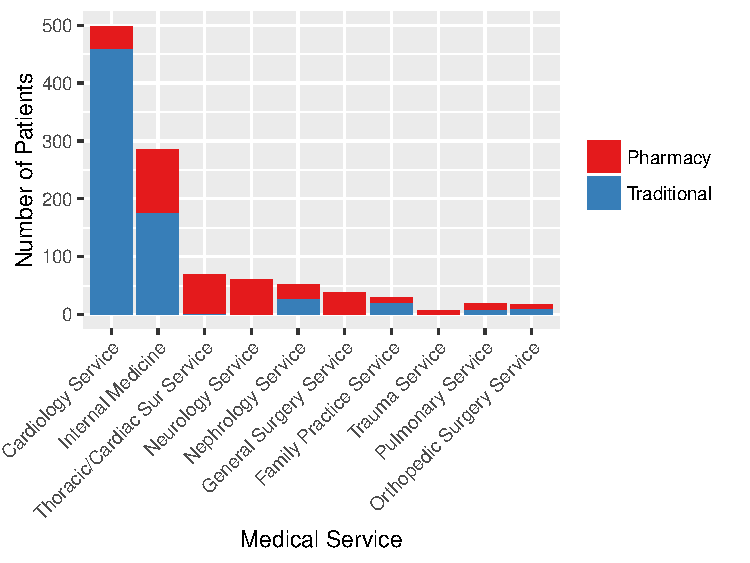
\includegraphics{warfarin_analysis_ASHP_files/figure-latex/ds_med_service_curr-1.pdf}
\caption{Warfarin Dosing Service Utilization Among Top 10 Medical
Services Ordering Warfarin}
\end{figure}

\subsection{Comparison}\label{comparison}

\begin{itemize}
\tightlist
\item
  Group 1 - Pharmacy Dosing Service

  \begin{itemize}
  \tightlist
  \item
    Consult placed within 48 hours of warfarin initiation
  \item
    At least 60\% of warfarin doses placed by pharmacist
  \end{itemize}
\item
  Group 2 - Traditional Dosing
\end{itemize}

\paragraph{Inclusion}\label{inclusion}

\begin{itemize}
\tightlist
\item
  January 1, 2015 to December 31, 2015
\item
  Age 18 years or greater
\item
  Received at least 3 doses of warfarin
\item
  Baseline INR \textless{} 1.5
\end{itemize}

\paragraph{Exclusion}\label{exclusion}

\begin{itemize}
\tightlist
\item
  Concurrent DTI or TSOAC
\item
  Liver dysfunction

  \begin{itemize}
  \tightlist
  \item
    AST and ALT \textgreater{} 5x ULN (concurrently)
  \item
    ALT \textgreater{} 10x ULN
  \item
    T.Bili \textgreater{} 3x ULN
  \end{itemize}
\item
  Missing goals of therapy data
\item
  Readmission encounters
\end{itemize}

\subsubsection{Results}\label{results}

\begin{longtable}[]{@{}llll@{}}
\caption{Demographics}\tabularnewline
\toprule
& pharmacy & traditional & p\tabularnewline
\midrule
\endfirsthead
\toprule
& pharmacy & traditional & p\tabularnewline
\midrule
\endhead
n & 402 & 285 &\tabularnewline
Age (median {[}IQR{]}) & 58.00 {[}42.25, 68.75{]} & 64.00 {[}54.00,
72.00{]} & \textless{}0.001\tabularnewline
Sex = Male (\%) & 240 (59.7) & 182 (64.1) & 0.279\tabularnewline
BMI (median {[}IQR{]}) & 28.48 {[}24.40, 33.54{]} & 29.32 {[}25.18,
33.68{]} & 0.277\tabularnewline
Race (\%) & & & 0.096\tabularnewline
- African American & 104 (28.4) & 74 (27.9) &\tabularnewline
- Asian & 12 ( 3.3) & 1 ( 0.4) &\tabularnewline
- Native Am. & 0 ( 0.0) & 1 ( 0.4) &\tabularnewline
- Other & 78 (21.3) & 59 (22.3) &\tabularnewline
- White/Caucasian & 172 (47.0) & 130 (49.1) &\tabularnewline
Length of Stay (median {[}IQR{]}) & 12.10 {[}7.71, 19.83{]} & 13.71
{[}8.04, 24.17{]} & 0.103\tabularnewline
Therapy = New/Previous (\%) & 270/132 (67.2/32.8) & 143/142 (50.2/49.8)
& \textless{}0.001\tabularnewline
\bottomrule
\end{longtable}

\begin{figure}[H]
\centering
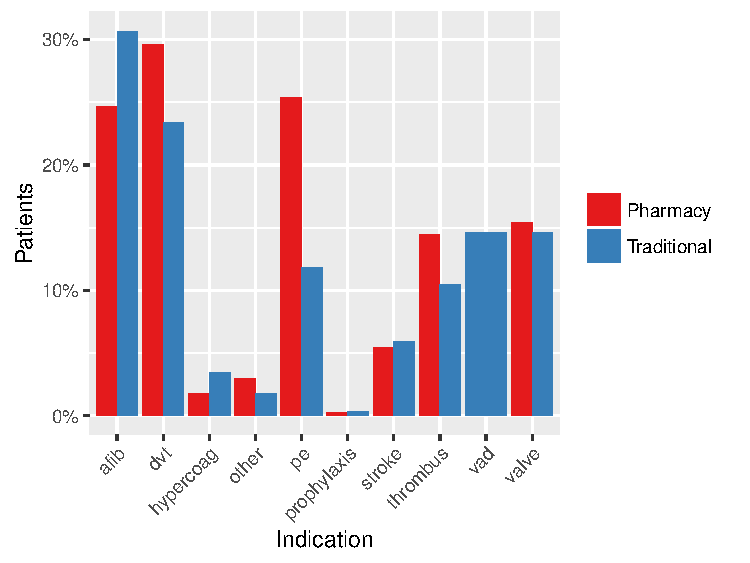
\includegraphics{warfarin_analysis_ASHP_files/figure-latex/indications-1.pdf}
\caption{Indications for warfarin use}
\end{figure}

\begin{figure}[H]
\centering
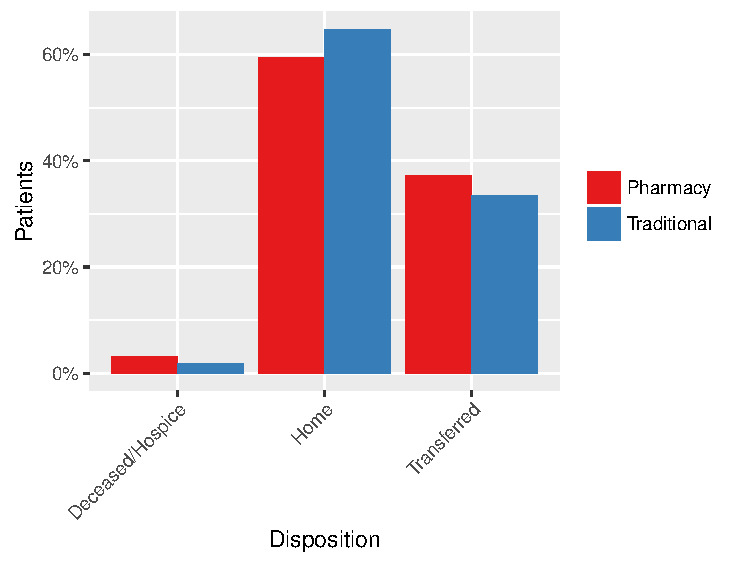
\includegraphics{warfarin_analysis_ASHP_files/figure-latex/disposition-1.pdf}
\caption{Disposition on discharge}
\end{figure}

\begin{figure}[H]
\centering
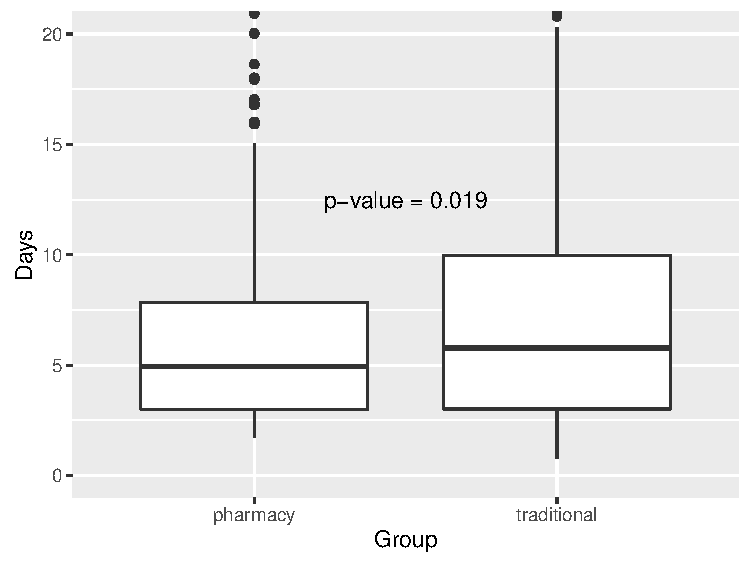
\includegraphics{warfarin_analysis_ASHP_files/figure-latex/dosing_days-1.pdf}
\caption{Inpatient Dosing Days}
\end{figure}

\subsubsection{Efficacy Endpoints}\label{efficacy-endpoints}

\begin{figure}[H]
\centering
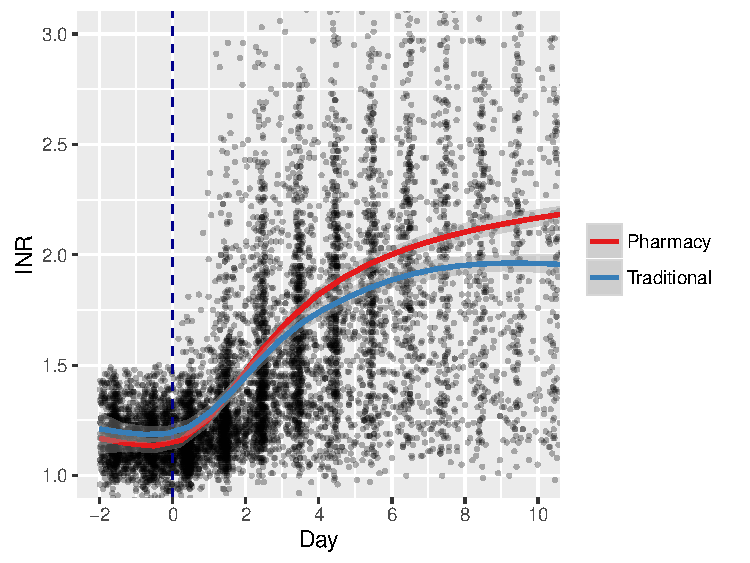
\includegraphics{warfarin_analysis_ASHP_files/figure-latex/inr-1.pdf}
\caption{INR response after starting warfarin}
\end{figure}

\begin{figure}[H]
\centering
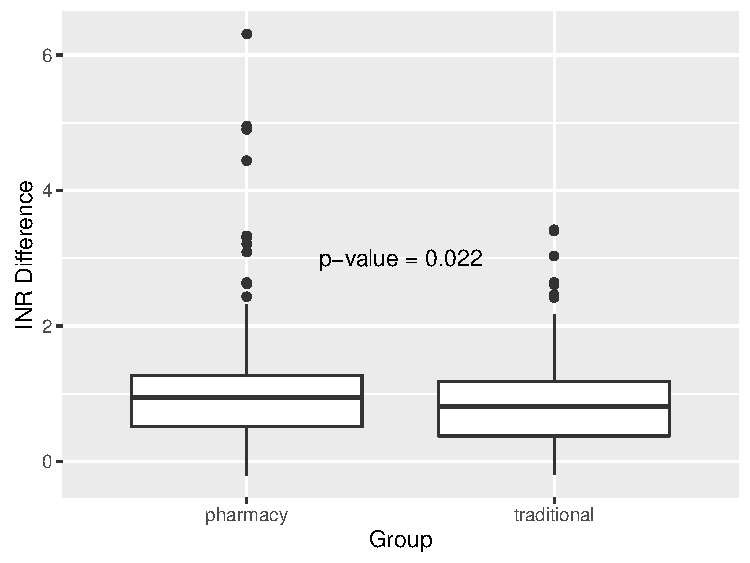
\includegraphics{warfarin_analysis_ASHP_files/figure-latex/inr2-1.pdf}
\caption{Change in INR}
\end{figure}

\begin{figure}[H]
\centering
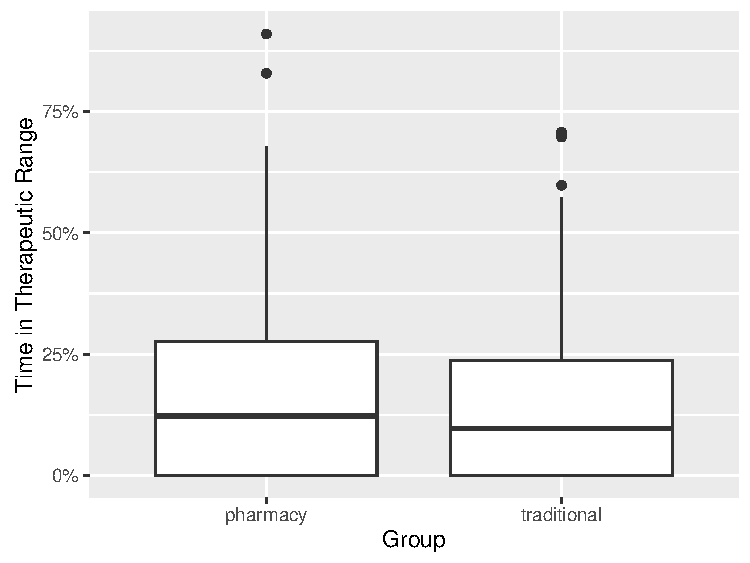
\includegraphics{warfarin_analysis_ASHP_files/figure-latex/ttr-1.pdf}
\caption{Percent of time INR is within therapeutic range}
\end{figure}

\subsubsection{Safety Endpoints}\label{safety-endpoints}

\begin{figure}[H]
\centering
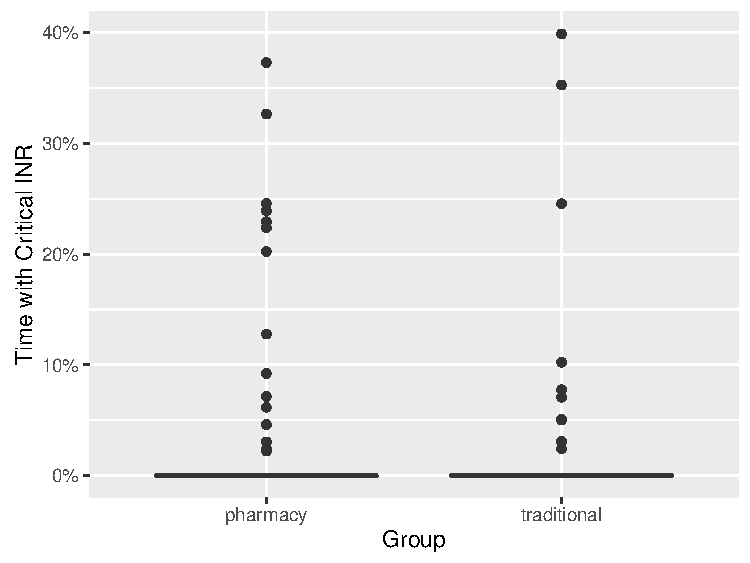
\includegraphics{warfarin_analysis_ASHP_files/figure-latex/time_above4-1.pdf}
\caption{Percent of time INR is critical (above 4)}
\end{figure}

\begin{figure}[H]
\centering
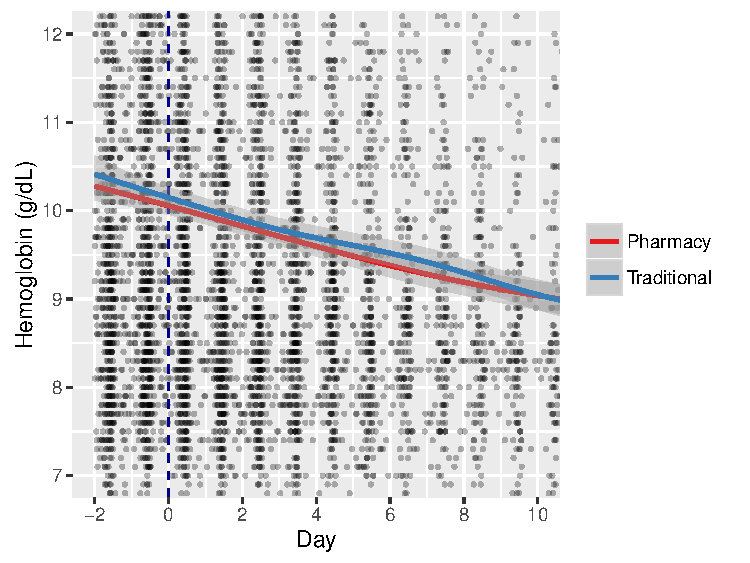
\includegraphics{warfarin_analysis_ASHP_files/figure-latex/hgb-1.pdf}
\caption{Change in hemoglobin after starting warfarin}
\end{figure}

\begin{figure}[H]
\centering
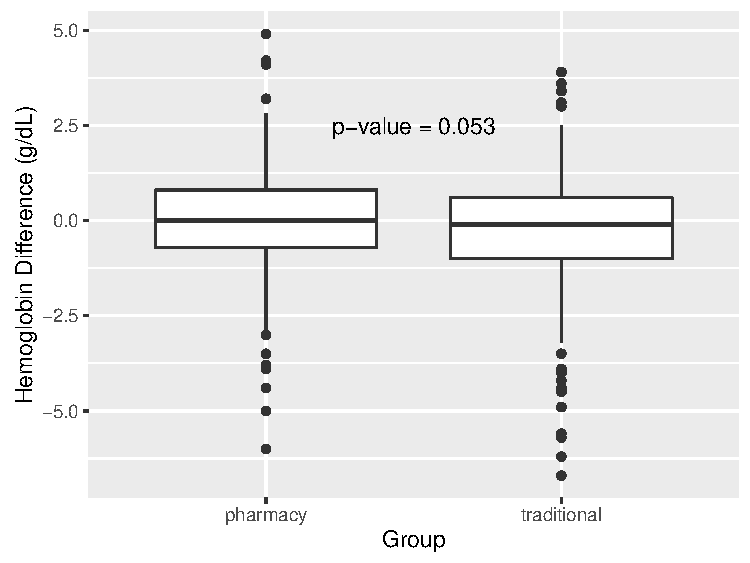
\includegraphics{warfarin_analysis_ASHP_files/figure-latex/hgb2-1.pdf}
\caption{Change in Hemoglobin}
\end{figure}

\subsection{Historical Comparison}\label{historical-comparison}

\begin{itemize}
\tightlist
\item
  Pharmacy Dosing Service 2015 vs.~2013-2014
\item
  Same inclusion and exclusion criteria
\end{itemize}

\begin{longtable}[]{@{}llll@{}}
\caption{Demographics}\tabularnewline
\toprule
& current & historical & p\tabularnewline
\midrule
\endfirsthead
\toprule
& current & historical & p\tabularnewline
\midrule
\endhead
n & 402 & 866 &\tabularnewline
Age (median {[}IQR{]}) & 58.00 {[}42.25, 68.75{]} & 59.00 {[}46.00,
71.00{]} & 0.048\tabularnewline
Sex = Male (\%) & 240 (59.7) & 505 (58.3) & 0.685\tabularnewline
BMI (mean (sd)) & 29.95 (8.50) & 29.90 (9.26) & 0.926\tabularnewline
Race (\%) & & & 0.189\tabularnewline
- African American & 104 (28.4) & 245 (31.2) &\tabularnewline
- Asian & 12 ( 3.3) & 15 ( 1.9) &\tabularnewline
- Latin American & 0 ( 0.0) & 1 ( 0.1) &\tabularnewline
- Other & 78 (21.3) & 133 (16.9) &\tabularnewline
- White/Caucasian & 172 (47.0) & 392 (49.9) &\tabularnewline
-Length of Stay (median {[}IQR{]}) & 12.10 {[}7.71, 19.83{]} & 11.85
{[}7.38, 18.62{]} & 0.172\tabularnewline
Therapy = New/Previous (\%) & 270/132 (67.2/32.8) & 604/262 (69.7/30.3)
& 0.390\tabularnewline
\bottomrule
\end{longtable}

\begin{figure}[H]
\centering
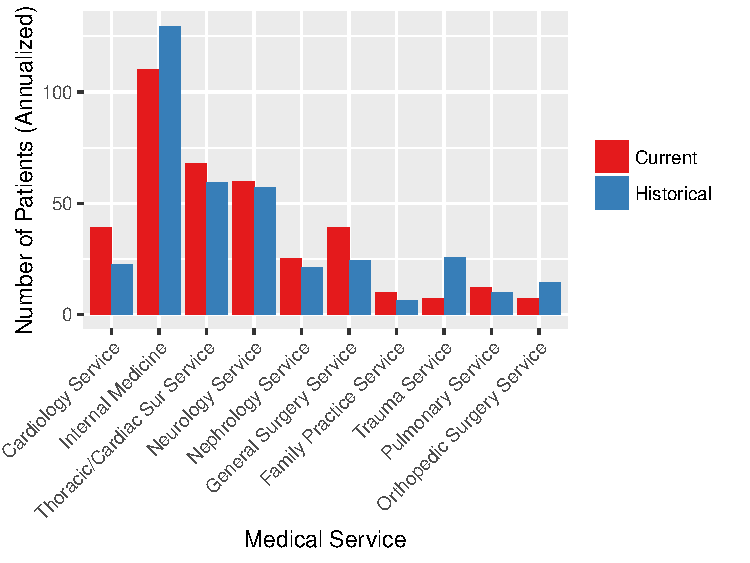
\includegraphics{warfarin_analysis_ASHP_files/figure-latex/ds_med_service-1.pdf}
\caption{Warfarin Dosing Service Utilization Among Top 10 Medical
Services Ordering Warfarin}
\end{figure}

\begin{figure}[H]
\centering
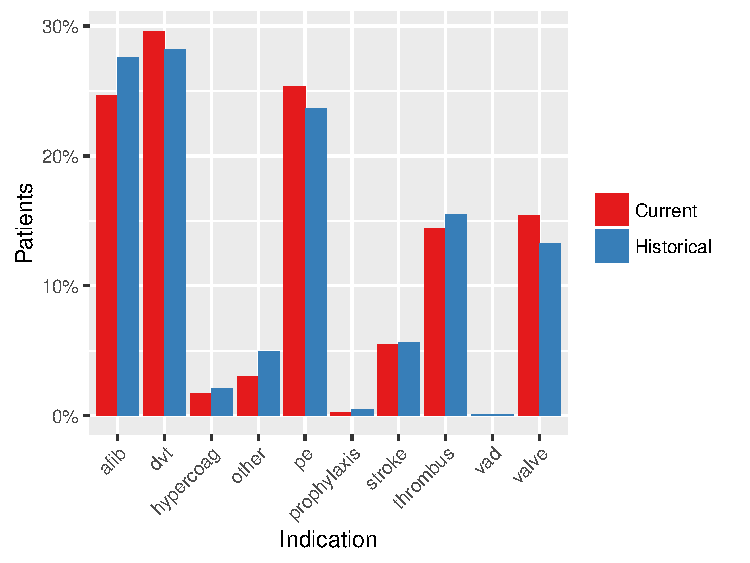
\includegraphics{warfarin_analysis_ASHP_files/figure-latex/indications_hist-1.pdf}
\caption{Indications for warfarin use}
\end{figure}

\begin{figure}[H]
\centering
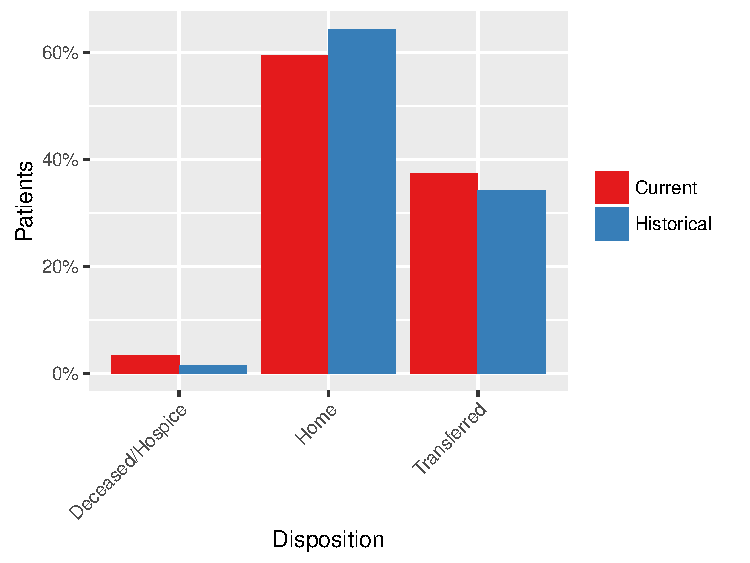
\includegraphics{warfarin_analysis_ASHP_files/figure-latex/disposition_hist-1.pdf}
\caption{Disposition on discharge}
\end{figure}

\begin{figure}[H]
\centering
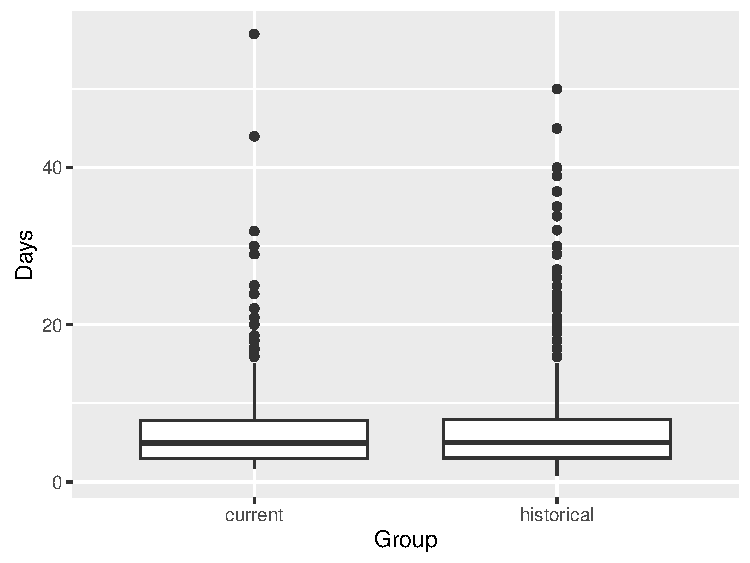
\includegraphics{warfarin_analysis_ASHP_files/figure-latex/dosing_days_hist-1.pdf}
\caption{Inpatient Dosing Days}
\end{figure}

\subsubsection{Efficacy Endpoints}\label{efficacy-endpoints-1}

\begin{figure}[H]
\centering
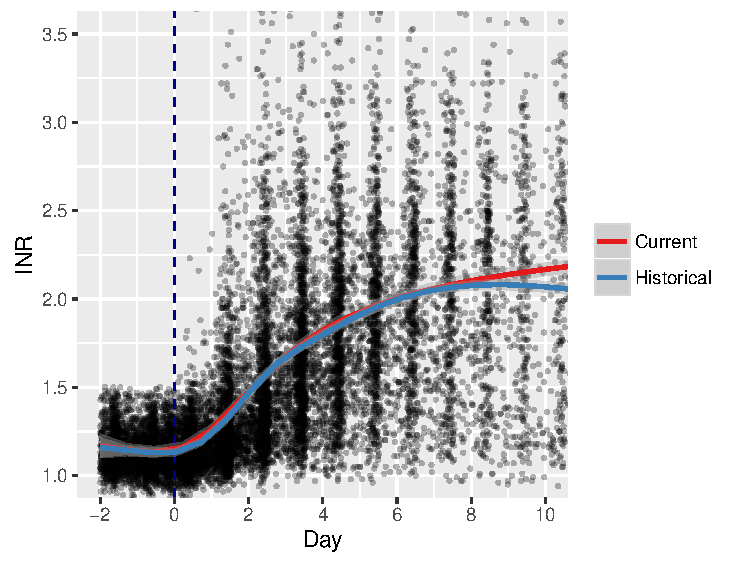
\includegraphics{warfarin_analysis_ASHP_files/figure-latex/inr_hist-1.pdf}
\caption{Change in INR after starting warfarin}
\end{figure}

\begin{figure}[H]
\centering
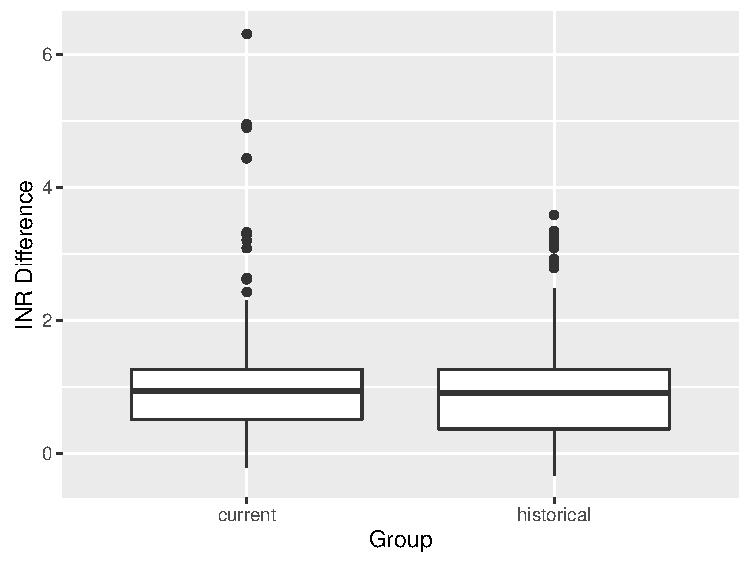
\includegraphics{warfarin_analysis_ASHP_files/figure-latex/inr2_hist-1.pdf}
\caption{Change in INR}
\end{figure}

\begin{figure}[H]
\centering
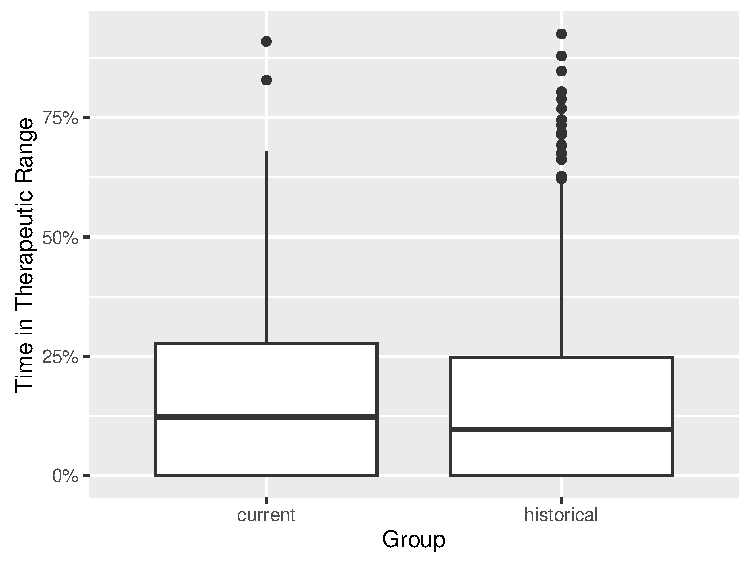
\includegraphics{warfarin_analysis_ASHP_files/figure-latex/ttr_hist-1.pdf}
\caption{Percent of time INR is within therapeutic range}
\end{figure}

\subsubsection{Safety Endpoints}\label{safety-endpoints-1}

\begin{figure}[H]
\centering
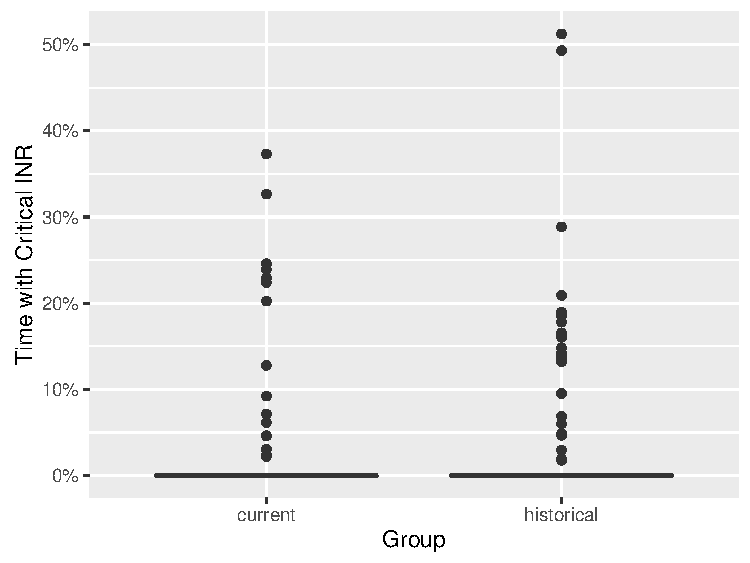
\includegraphics{warfarin_analysis_ASHP_files/figure-latex/critical_hist-1.pdf}
\caption{Percent of time INR is critical (above 4)}
\end{figure}

\begin{figure}[H]
\centering
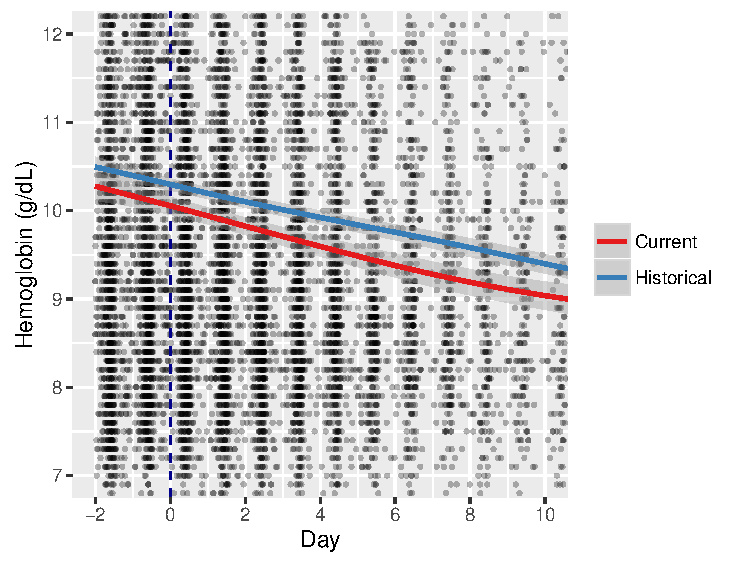
\includegraphics{warfarin_analysis_ASHP_files/figure-latex/hgb_hist-1.pdf}
\caption{Change in hemoglobin after starting warfarin}
\end{figure}

\begin{figure}[H]
\centering
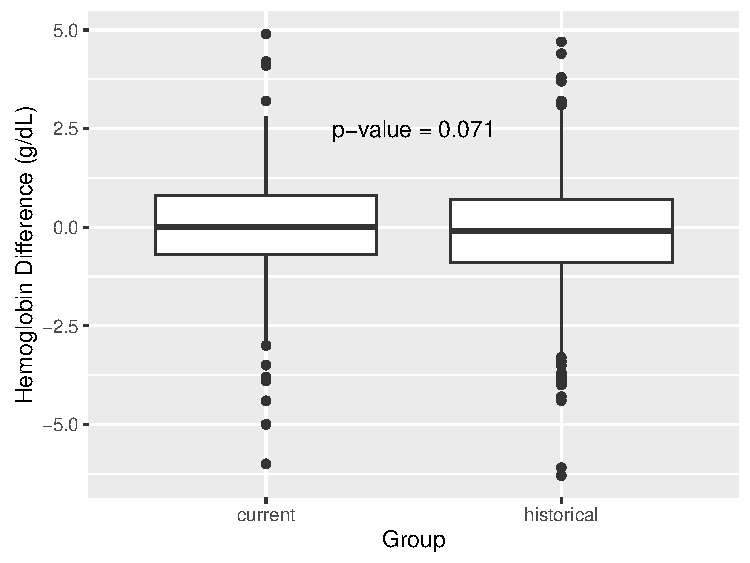
\includegraphics{warfarin_analysis_ASHP_files/figure-latex/hgb2_hist-1.pdf}
\caption{Change in Hemoglobin}
\end{figure}


\end{document}
